% file: circular-queue-array.tex

\documentclass[tikz]{standalone}
\usetikzlibrary{decorations.pathreplacing, positioning, arrows.meta, shapes.multipart}

\begin{document}
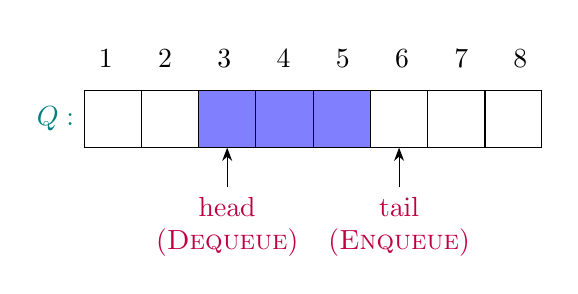
\begin{tikzpicture}[Array/.style = {rectangle split, rectangle split parts = #1, rectangle split horizontal,
    inner sep = 8pt, anchor = center}]
  % the queue
  \node[Array = {8}, draw, rectangle split part fill = {white, white, blue!50, blue!50, blue!50, white}, label = {left: \textcolor{teal}{$Q:$}}] (Q) 
    {\nodepart{two} \nodepart{three} \nodepart{four} \nodepart{five} \nodepart{six} \nodepart{seven} \nodepart{eight}};
  % queue index
  \node[Array = {8}, above = 0.cm of Q] (Q-index) 
    {1\nodepart{two}2\nodepart{three}3\nodepart{four}4\nodepart{five}5\nodepart{six}6\nodepart{seven}7\nodepart{eight}8};

  % head
  \node[below = 0.50cm of Q.three south, align = center, purple] (head) {head \\ (\textsc{Dequeue})};
  \draw[->, >= Stealth] (head) to (Q.three south);

  % tail
  \node[below = 0.50cm of Q.six south, align = center, purple] (tail) {tail \\ (\textsc{Enqueue})};
  \draw[->, >= Stealth] (tail) to (Q.six south);
\end{tikzpicture}
\end{document}